\subsection{Umfrage}
Um das Konzept über und um den Fahrradturm an die zukünftig Benutzenden anzupassen hat das Projektteam eine Umfrage erstellt. 257 Personen haben geantwortet, die jüngste Person war 15 Jahre alt, die älteste Person war 82 Jahre. Folgende Altersgruppen waren vertreten:


\begin{table}[H]
    \centering
    \begin{tabular}{lr}
        \toprule
        Altersgruppe  & Anzahl Personen \\
        \midrule
        0 - 20 Jahre  & 9               \\
        21 - 30 Jahre & 91              \\
        31 - 40 Jahre & 76              \\
        41 - 50 Jahre & 35              \\
        51 - 60 Jahre & 28              \\
        61 - 82 Jahre & 18              \\
        \bottomrule
    \end{tabular}
    \caption{Verteilung der Umfrageteilnehmer nach Alter}
    \label{tab:umfragealter}
\end{table}

Geographische verteilt sich die Herkunft der Umfrageteilnehmer auf 4 Staaten, dies waren Österreich, Deutschland, Schweiz und ein anderes Land. Den größten Anteil davon haben mit 240 die Deutschen, gefolgt von 14 Österreichern, zwei Schweizern und 1 anderen Staatsbewohner.\\
Von den 256 Fahrradbesitzern nutzen 49 ein E-Bike, d.h. die Mehrzahl nutzt noch ein normales Fahrrad.\\
\begin{figure}[H]
    \centering
    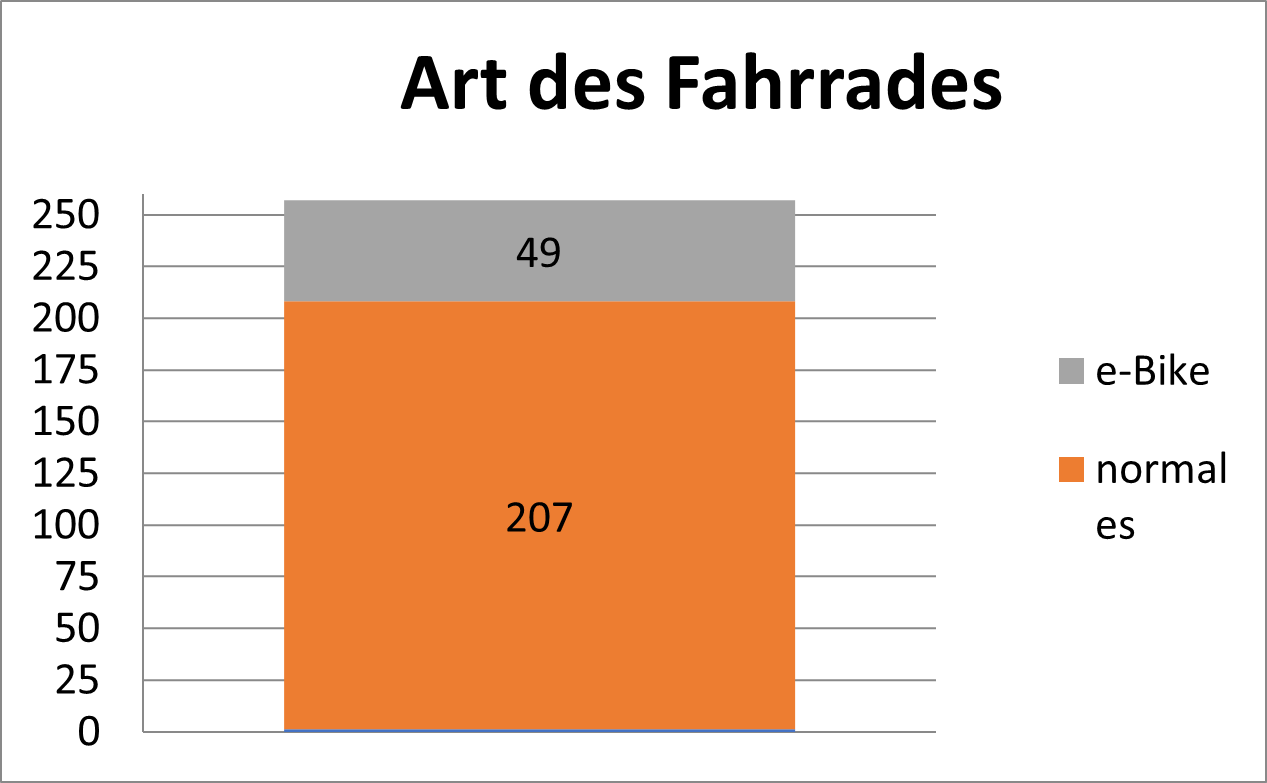
\includegraphics[width=0.4\textwidth]{images/artdesfahrrades.png}
    \caption{Diagramm Fahrrad-Typ}
    \label{fig:diagrammfahrradtyp}
\end{figure}
Unter den E-Bike Radfahrer könnten sich 28 Personen vorstellen, den Biketower zu nutzen, hier ist die die Zustimmung mit 57 \% höher, als bei den Normalrad-Fahrer, wo sich nur 47 \% vorstellen können das System zu nutzen, auch die definitive Ablehnung ist hier höher.\\
\begin{figure}[H]
    \centering
    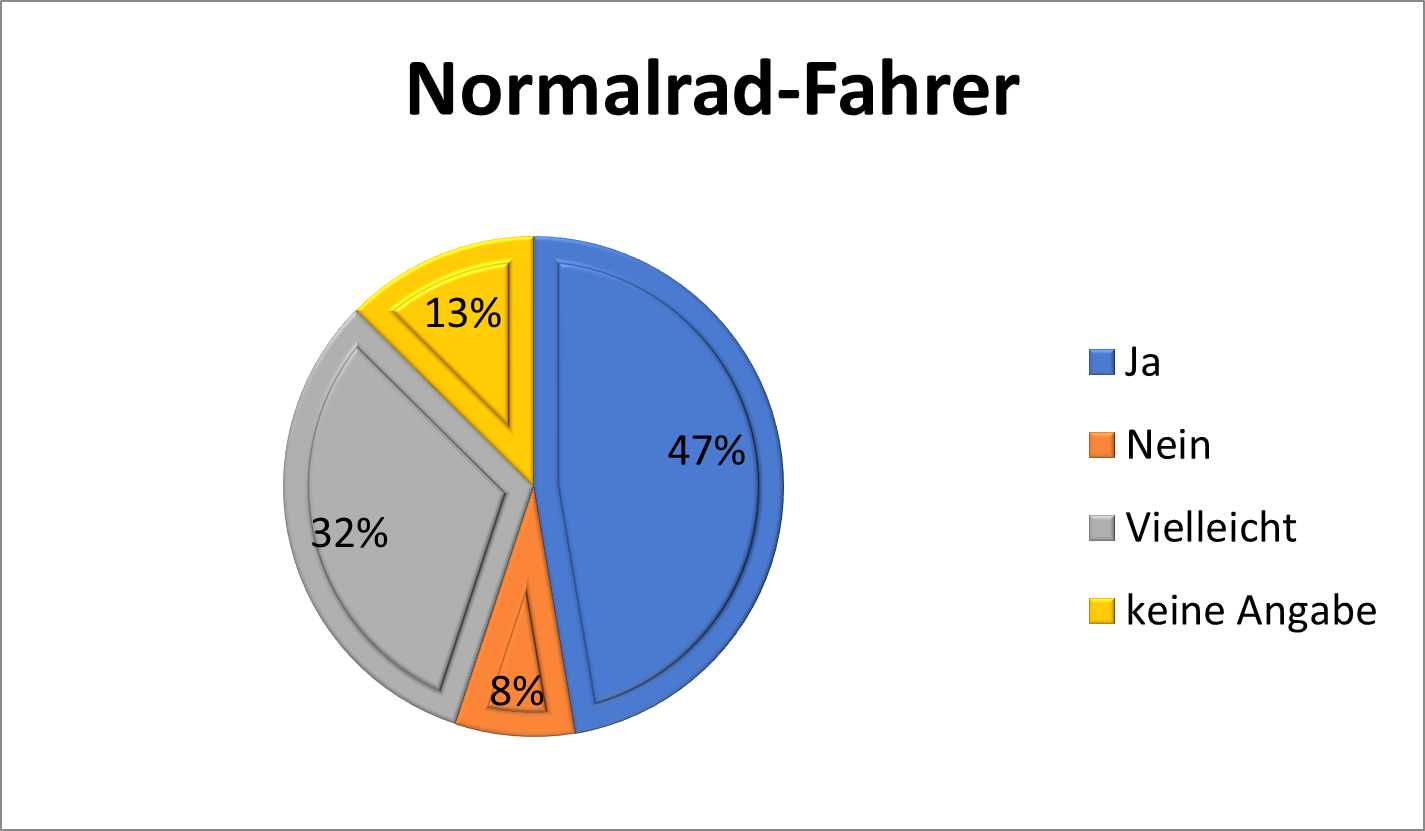
\includegraphics[width=0.35\textwidth]{images/normalradfahrer.png}
    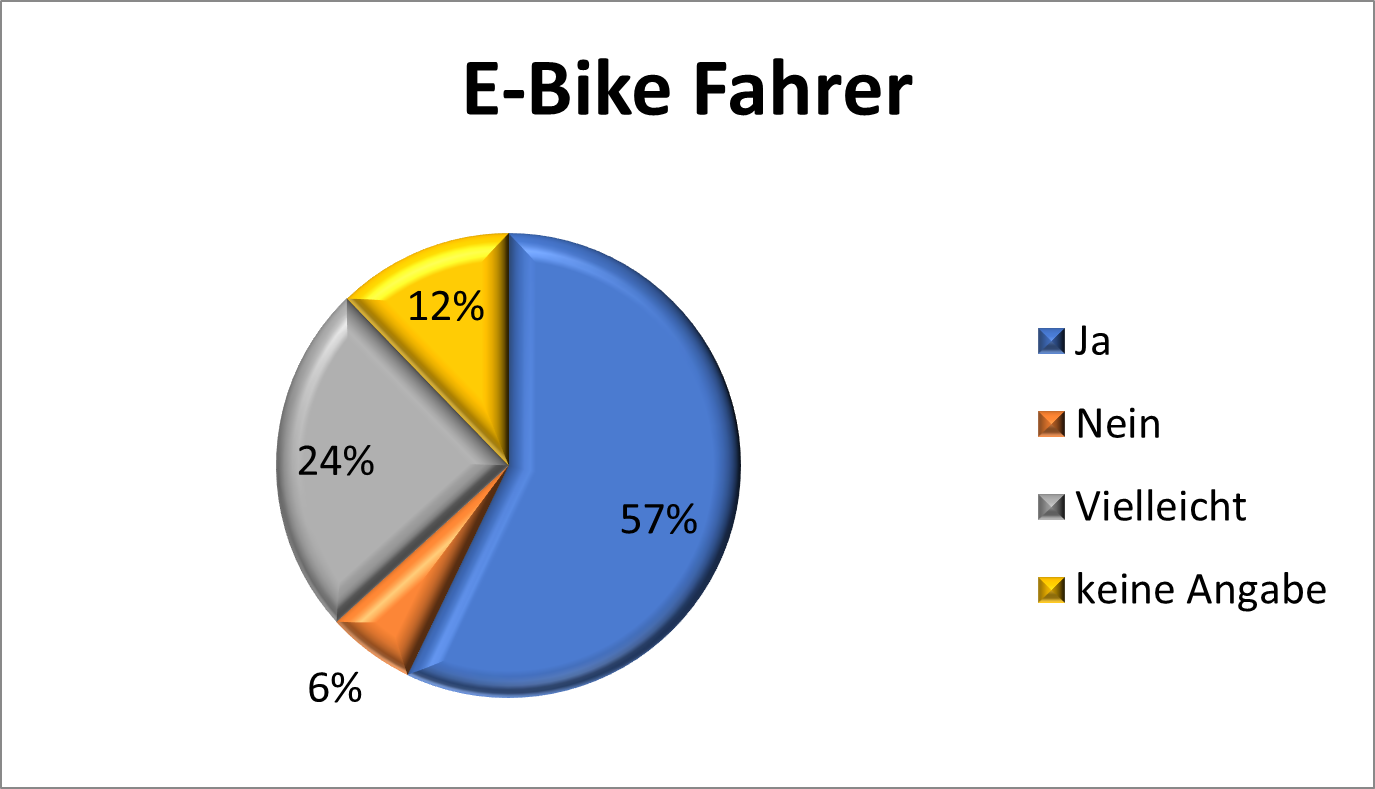
\includegraphics[width=0.35\textwidth]{images/ebikefahrer.png}
    \caption{Bereitschaft ein automatisches Fahrradparksystem zu verwenden}
    \label{fig:bereitschaftnutzung}
\end{figure}
Bei den 256 Fahrradbesitzern verwendet die Mehrzahl, in Summe 132 Personen, ein Fahrrad in der Preisklasse von € 1.000 – € 3.0000, die zweitgrößte Gruppe nutzt ein Fahrrad in der Preisspanne von € 0 bis € 1.000. Mehr als 53 Personen benutzen ein Fahrrad, das mehr als € 3.000,-- gekostet hat.\\
\begin{figure}[H]
    \centering
    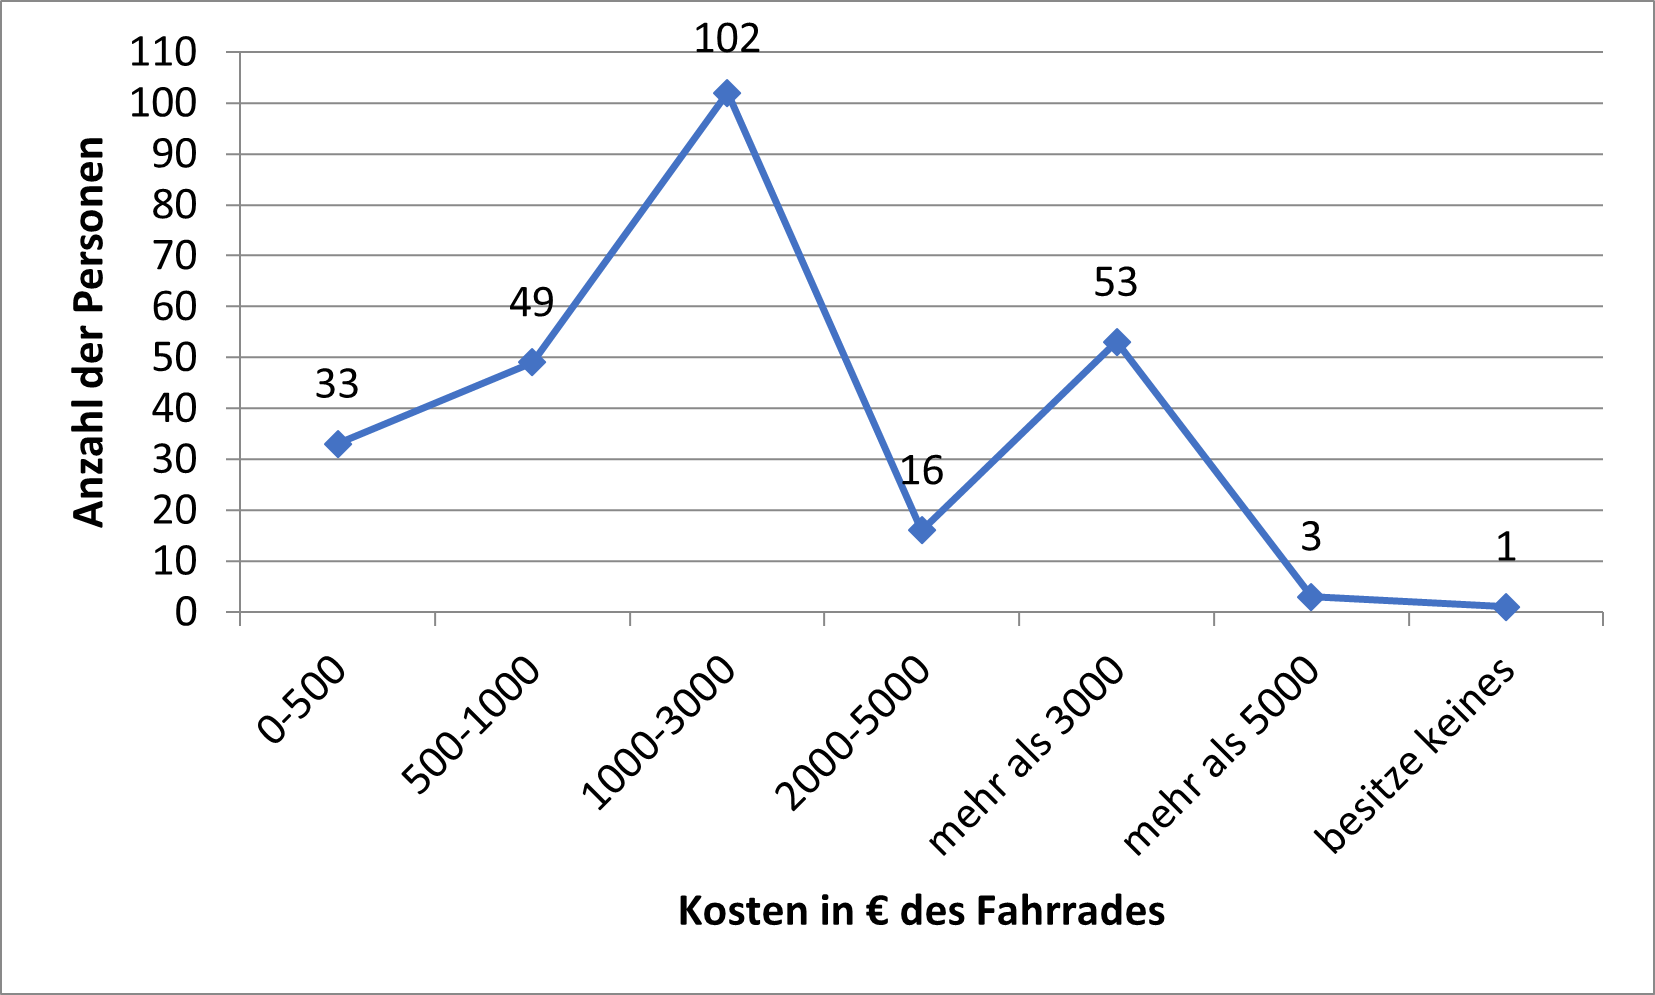
\includegraphics[width=0.4\textwidth]{images/fahrradkosten.png}
    \caption{Durchschnittliche Fahrradkosten}
    \label{fig:fahrradkosten}
\end{figure}
Auch das Nutzungsverhalten verteilt sich höchst unterschiedlich, 6 Personen nutzen ihr Fahrrad nur einmal pro Monat, davon 3 hauptsächlich für Freizeitaktivitäten, 2 für Einkaufen und Freizeitaktivitäten und eine Person für den Arbeitsweg und Freizeitaktivititäten. Einmal pro Woche nutzen 15 Personen ihr Fahrrad größtenteils für Einkaufen, Freizeitaktivitäten und 5 davon fahren mindestens 1 x wöchentlich damit zur Arbeit. 9 Personen verwenden ihr Fahrrad ausschließlich für den Arbeitsweg.\\
183 Personen verwenden das Fahrrad vorrangig für den Arbeitsweg, 30 primär für das Einkaufen und 43 am häufigsten für die Freizeitaktivitäten. Hier handelt es sich um Angabe der primären und erstrangigen Verwendung, auch die berufspendelnden Radler verwenden ihr Fahrrad noch zum Einkaufen, für Freizeitaktivitäten u.s.w., es wird nur erstrangig angegeben.\\
Innerhalb dieser Gruppen ist die Vorstellung, einen Biketower zu nutzen wieder sehr unterschiedlich verteilt.\\
In allen drei Verwendungsgruppen überwiegt die Vorstellung, ein Automatisches Fahrradparksystem zu nutzen, prozentmäßig am stärksten kann es sich die Verwendungspruppe, die das Fahrrad primär zum Einkaufen und vor allen anderen Aktivitäten nutzt, vorstellen, gefolgt von der Gruppe vorwiegend Freizeitaktivität nutzende Radfahrer, und jenen Radfahrer die vor allem das Fahrrad für den Arbeitsweg benützen. Auffällig ist, dass sich in der Gruppe der Arbeitsweg-Radler am meisten nicht vorstellen können, das Angebot eines vollautomatisierten Biketowers zu nutzen. Wobei auch hier die Nicht-Vorstellung am letzten Platz liegt, nach der Zustimmung, der Vielleicht-Benutzung und den leeren Angaben. Nur 19 Personen aus allen Verwendungsgruppen lehnen die Vorstellung der Benutzung vollkommen ab.\\





